% Metódy inžinierskej práce -- predbežná verzia projektu
% Formulár VV-F -- vecný zámer projektu (záväzná osnova APVV VV 2024, max. 15 strán)
\documentclass[11pt,a4paper]{article}

\usepackage[slovak]{babel}
\usepackage[T1]{fontenc}
\usepackage[utf8]{inputenc}
\usepackage{newtxtext,newtxmath} % Times New Roman
\usepackage[margin=2.2cm]{geometry}
\usepackage{graphicx}
\usepackage{tabularx}
\usepackage{booktabs}
\usepackage{xcolor}
\usepackage{fancyhdr}
\usepackage{url}
\usepackage[hidelinks]{hyperref}
\usepackage{cite}

\newcommand{\akronym}{AI-PENTEST}
\newcommand{\doplnit}[1]{\textcolor{gray}{[#1]}}
\newcommand{\bod}[1]{\subsection*{#1}}

\pagestyle{fancy}
\fancyhf{}
\lhead{\small VV-F -- Vecný zámer projektu}
\rhead{\small Akronym: \akronym}
\cfoot{\small \thepage}
\setlength{\headheight}{14pt}

\begin{document}

\begin{center}
  {\Large\bfseries VV-F -- VECNÝ ZÁMER PROJEKTU}\\[2pt]
  {\small Záväzná osnova pre aplikovaný výskum a vývoj (VV 2024)}\\[2pt]
  {\small Predbežná verzia, Metódy inžinierskej práce, ak. rok 2026/27}
\end{center}

\noindent
\begin{tabularx}{\textwidth}{@{}lX@{}}
\toprule
\textbf{Názov projektu} & Inteligentný systém na automatizované testovanie bezpečnosti webových aplikácií pomocou veľkých jazykových modelov (\akronym) \\
\textbf{Zodpovedný riešiteľ} & Andrii Tsybulskyi \\
\textbf{Riešitelia} & Kyrylo Bukhanets, Artur Toba, Maksym Tomkevych \\
\textbf{Žiadateľ} & Slovenská technická univerzita v~Bratislave, Fakulta informatiky a informačných technológií \\
\bottomrule
\end{tabularx}

% =================================================================
\section{Excelentnosť}

\bod{Projektový zámer, navrhovaný spôsob riešenia a aplikačná úroveň očakávaných výsledkov}
Penetračné testovanie webových aplikácií je dnes prevažne manuálna a drahá činnosť. Automatizované skenery sú rýchle, no zraniteľnosti viazané na logiku a stav aplikácie často prehliadnu~\cite{Doupe-Johnny}. Veľké jazykové modely (LLM) a agentné systémy postavené nad nimi ukazujú, že dokážu plánovať test, ovládať bežné nástroje a v~niektorých prípadoch samostatne zneužiť zraniteľnosť~\cite{Deng-PentestGPT,Fang-HackWebsites}. Chýba však spoločné, bezpečné a opakovateľné prostredie, v~ktorom by sa schopnosti takýchto agentov dali objektívne porovnať.

Projekt \akronym{} preto vytvorí \textbf{Web Pentest Harness} -- kontrolované prostredie, v~ktorom AI agent dostane prístup k~zámerne zraniteľnej webovej aplikácii a pokúsi sa ju samostatne otestovať. Harness:
\begin{itemize}
  \item spúšťa testované aplikácie v~izolovaných kontajneroch bez prístupu na internet,
  \item poskytuje agentovi jednotnú sadu nástrojov (HTTP klient, prehliadač, skener, terminál v~sandboxe),
  \item zaznamenáva každú akciu agenta a pred jej vykonaním kontroluje povolený rozsah,
  \item overuje nahlásené zraniteľnosti kontrolovaným proof-of-concept postupom,
  \item porovnáva nálezy s~referenčnou databázou a počíta hodnotiace metriky.
\end{itemize}
Očakávané výsledky sú na úrovni overenia technológie v~relevantnom prostredí (TRL~5): funkčný softvér, verejný benchmark a metodika hodnotenia, ktoré môžu priamo použiť výskumné tímy, bezpečnostné firmy aj vyučujúci.

\bod{Aktuálnosť cieľov a originalita projektu}
Bezpečnosť webových aplikácií zostáva kritickou oblasťou -- kategórie OWASP Top 10 sa v~praxi opakovane objavujú~\cite{OWASP-Top10}. Súčasne prudko rastú schopnosti AI agentov a s~nimi aj potreba merať ich prínos aj riziká, čo zdôrazňujú aj odporúčania NIST pre hodnotenie AI systémov~\cite{NIST-AIME,NIST-ARIA}.

Originalita projektu spočíva v~troch bodoch: (1) harness hodnotí nielen to, \emph{či} agent uspel, ale aj \emph{ako} -- presnosť, úplnosť, falošné nálezy, čas a náklady; (2) každý nález sa automaticky overuje, takže výsledky nezávisia od tvrdení samotného modelu; (3) benchmark obsahuje aj vlastné, nepublikované zraniteľnosti, čím sa obmedzí skreslenie spôsobené tým, že model mohol verejné úlohy vidieť pri trénovaní. Existujúce benchmarky typu \emph{capture the flag}, napríklad Cybench~\cite{Zhang-Cybench}, sa sústreďujú na nájdenie vlajky, nie na úplnosť nálezov v~reálnej webovej aplikácii.

\bod{Stav poznania, vedecké základy a predchádzajúce výsledky}
Metodickým základom testovania je OWASP Web Security Testing Guide~\cite{OWASP-WSTG}. Klasické nástroje statickej (SAST) a dynamickej (DAST) analýzy, napríklad ZAP~\cite{ZAP}, poskytujú rýchlu, no plytkú kontrolu. Prvé práce s~LLM ukázali, že modely zvládajú jednotlivé kroky penetračného testu, no strácajú kontext pri dlhých úlohách; PentestGPT to rieši rozdelením na moduly uvažovania, generovania a spracovania výstupov~\cite{Deng-PentestGPT}. Autonómni agenti dokázali v~izolovanom prostredí zneužiť viaceré typy webových zraniteľností~\cite{Fang-HackWebsites}. Ako cieľové aplikácie sa bežne používajú zámerne zraniteľné systémy, napríklad OWASP WebGoat~\cite{OWASP-WebGoat}. Podrobný prehľad je obsahom sprievodného prehľadového článku.

\bod{Ciele projektu a reálnosť ich dosiahnutia}
\begin{description}
  \item[C1 -- Harness.] Navrhnúť a implementovať Web Pentest Harness s~izoláciou, záznamom akcií a kontrolou rozsahu. \emph{Ukazovateľ:} 100\,\% akcií agenta zaznamenaných, 0 únikov mimo izolovanej siete počas experimentov.
  \item[C2 -- Benchmark.] Vytvoriť aspoň 40 úloh v~minimálne 8 triedach zraniteľností s~anotovanou referenčnou databázou; aspoň 25\,\% úloh bude nepublikovaných.
  \item[C3 -- Hodnotenie.] Implementovať hodnotiaci modul s~metrikami presnosť $P$, úplnosť $R$, $F_1$, miera falošných nálezov, medián času do nálezu a cena behu.
  \item[C4 -- Porovnanie.] Porovnať aspoň 4 architektúry agentov a 3 jazykové modely s~klasickým DAST nástrojom; každú konfiguráciu spustiť aspoň 5-krát.
\end{description}
Ciele sú reálne: využívajú existujúce otvorené technológie (kontajnery, zraniteľné aplikácie, API modelov) a tím ich overí najprv na pilotnej verzii s~niekoľkými úlohami.

\bod{Metodológia riešenia a jej opodstatnenosť}
Riešenie postupuje iteratívne. V~každej iterácii sa rozšíri benchmark, spustia sa experimenty a podľa výsledkov sa upraví harness.

\begin{enumerate}
  \item \textbf{Návrh architektúry.} Oddelenie agenta, nástrojov, testovanej aplikácie a hodnotiaceho modulu, aby sa dali vymieňať nezávisle.
  \item \textbf{Tvorba úloh.} Každá úloha obsahuje kontajner s~aplikáciou, zoznam zraniteľností (typ, URL, parameter, závažnosť) a skript na overenie.
  \item \textbf{Experimenty.} Agent dostane iba URL a popis rozsahu. Harness zaznamená priebeh a výsledné nálezy.
  \item \textbf{Vyhodnotenie.} Nález je správny (TP), ak sa zhoduje s~referenčnou zraniteľnosťou v~type aj umiestnení. Z~počtov TP, FP a FN sa vypočíta
  \[ P=\frac{TP}{TP+FP},\qquad R=\frac{TP}{TP+FN},\qquad F_1=\frac{2PR}{P+R}. \]
  Výsledky sa uvádzajú ako priemer a smerodajná odchýlka cez opakované behy.
\end{enumerate}
Zvolený postup je opodstatnený, pretože jediný spoľahlivý spôsob, ako porovnať nedeterministické systémy, je opakované meranie na rovnakých úlohách s~nezávislým overením výsledku.

\paragraph{Architektúra riešenia.} Navrhovanú architektúru znázorňuje obr.~\ref{fig:arch}. Riadiaci modul spúšťa beh: pripraví kontajner s~testovanou aplikáciou, odovzdá agentovi popis úlohy a sprístupní mu nástroje. Každé volanie nástroja prechádza cez \emph{kontrolór rozsahu}, ktorý odmietne akcie mimo povolenej adresy alebo akcie označené ako deštruktívne. Všetky volania a odpovede sa ukladajú do \emph{záznamu behu}. Po skončení behu \emph{overovací modul} pre každý nahlásený nález spustí overovací skript úlohy a \emph{hodnotiaci modul} porovná overené nálezy s~referenčnou databázou.

\begin{figure}[htbp]
  \centering
  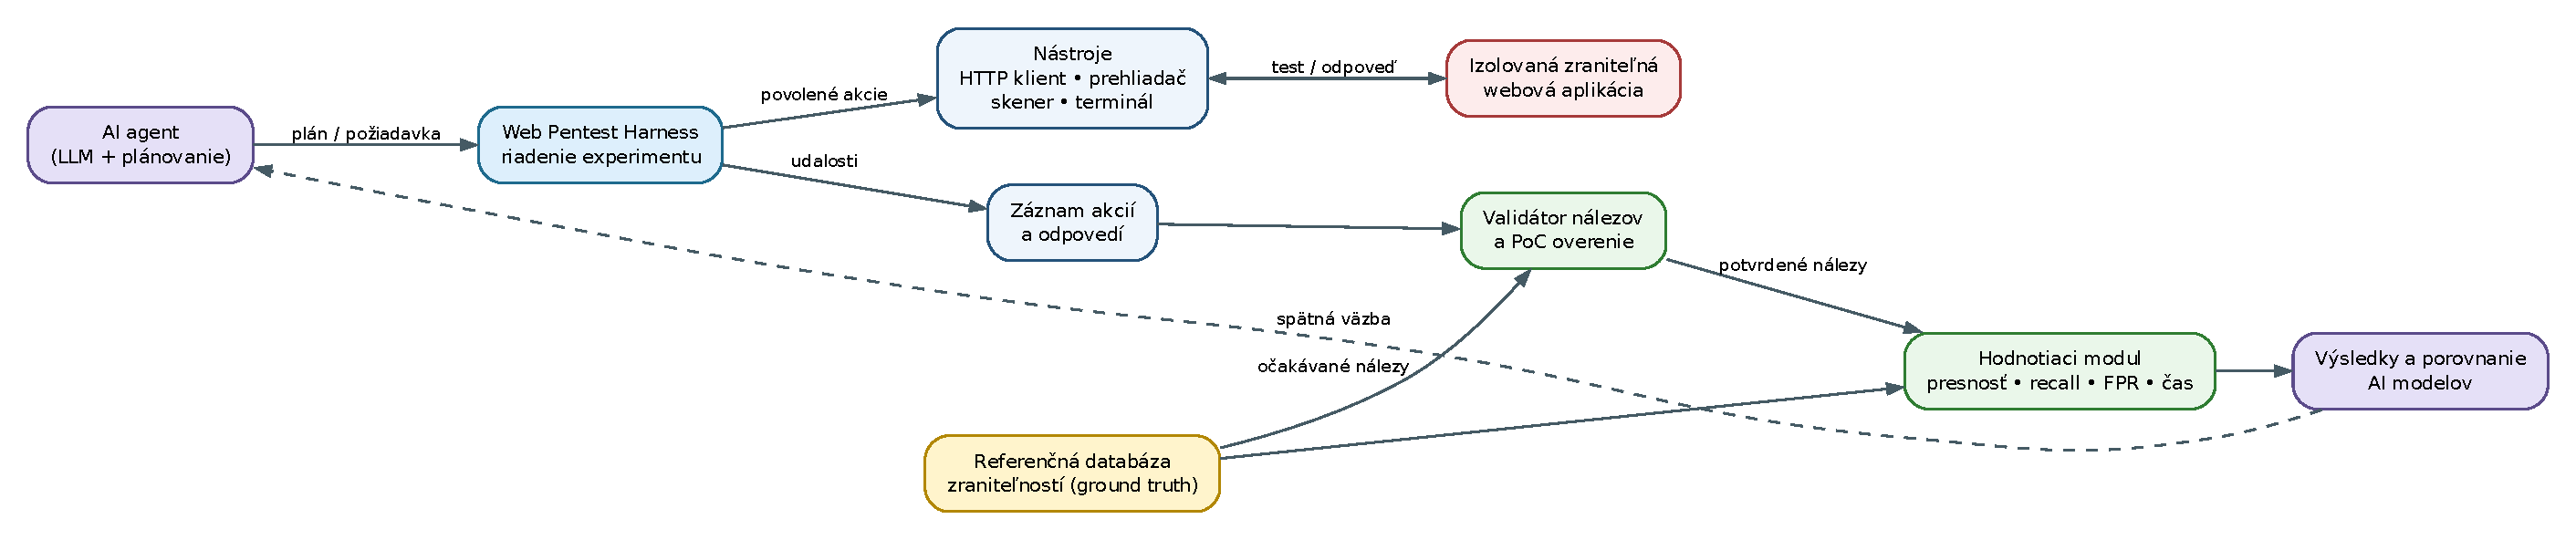
\includegraphics[width=0.95\textwidth]{../clanok/obrazky/diagram-architektura.pdf}
  \caption{Architektúra prostredia Web Pentest Harness.}
  \label{fig:arch}
\end{figure}

\paragraph{Taxonómia benchmarku.} Úlohy budú pokrývať hlavné kategórie OWASP Top 10~\cite{OWASP-Top10} v~troch úrovniach obtiažnosti. Plánované rozloženie uvádza tab.~\ref{tab:benchmark}. Ľahká úloha obsahuje jednu priamo dostupnú zraniteľnosť, stredná vyžaduje viac krokov (napr. prihlásenie), ťažká kombináciu viacerých chýb alebo porozumenie logike aplikácie.

\begin{table}[htbp]
\centering
\caption{Plánované rozloženie úloh benchmarku.}
\label{tab:benchmark}
\begin{tabular}{@{}lcccc@{}}
\toprule
\textbf{Trieda zraniteľnosti} & \textbf{Ľahká} & \textbf{Stredná} & \textbf{Ťažká} & \textbf{Spolu} \\ \midrule
SQL injection & 2 & 2 & 1 & 5 \\
Cross-site scripting (XSS) & 2 & 2 & 1 & 5 \\
Obchádzanie autentifikácie & 1 & 2 & 2 & 5 \\
Chybná autorizácia (IDOR) & 1 & 2 & 2 & 5 \\
Server-side request forgery (SSRF) & 1 & 2 & 2 & 5 \\
Nesprávna konfigurácia & 2 & 2 & 1 & 5 \\
Zraniteľné komponenty & 2 & 2 & 1 & 5 \\
Chyby v~logike aplikácie & 1 & 2 & 2 & 5 \\ \midrule
\textbf{Spolu} & \textbf{12} & \textbf{16} & \textbf{12} & \textbf{40} \\ \bottomrule
\end{tabular}
\end{table}

\paragraph{Návrh experimentov.} Porovnávať sa budú tieto konfigurácie: (A) klasický DAST nástroj ako referencia, (B) LLM v~úlohe asistenta, ktorý navrhuje kroky a nástroje vykonáva skript, (C) jednoduchý autonómny agent s~cyklom ,,uvažuj -- konaj -- pozoruj``, (D) modulárny agent s~oddeleným plánovaním a spracovaním výstupov podľa vzoru~\cite{Deng-PentestGPT} a (E) agent s~dlhodobou pamäťou nálezov. Konfigurácie B--E sa spustia s~troma jazykovými modelmi (dva komerčné, jeden otvorený). Každá kombinácia beží na každej úlohe aspoň päťkrát s~rovnakým časovým a tokenovým limitom, čo pri 40 úlohách dáva približne $4 \times 3 \times 40 \times 5 = 2\,400$ behov agentov.

\paragraph{Štatistické spracovanie.} Rozdiely medzi konfiguráciami sa budú testovať párovými neparametrickými testami na úrovni úloh, pretože rozdelenie úspešnosti nie je normálne. Okrem súhrnných metrík sa ručne analyzuje vzorka neúspešných behov a zlyhania sa zatriedia (napr. strata kontextu, opakovanie rovnakej akcie, halucinovaný nález), čo prinesie kvalitatívny pohľad na slabiny agentov.

\paragraph{Bezpečnosť a etika experimentov.} Autonómny agent schopný zneužiť zraniteľnosť je nástrojom dvojakého použitia. Projekt preto stanovuje tieto pravidlá:
\begin{itemize}
  \item experimenty bežia výlučne v~sieťovo izolovanom prostredí; agent nemá prístup na internet ani do siete univerzity,
  \item testujú sa iba aplikácie vytvorené alebo zámerne upravené na účely projektu, nikdy nie systémy tretích strán,
  \item kontrolór rozsahu blokuje akcie mimo povolených adries a operácie, ktoré by mohli poškodiť infraštruktúru (mazanie dát, zahltenie služby),
  \item záznamy behov neobsahujú osobné údaje, keďže aplikácie pracujú iba so syntetickými dátami,
  \item zverejňuje sa benchmark a metodika, nie postupy útoku na konkrétne reálne systémy.
\end{itemize}
Postup bude pred začatím experimentov konzultovaný s~etickou komisiou žiadateľa.

\bod{Najdôležitejšie výstupy zodpovedného riešiteľa za posledných 5 rokov}
Zodpovedný riešiteľ je mladý výskumný pracovník na začiatku kariéry a zatiaľ nemá aplikačné výstupy.

\bod{Najdôležitejšie projekty zodpovedného riešiteľa za posledných 5 rokov}
Žiadne. Projekt je prvým samostatným projektom tímu.

\bod{Kvalita zodpovedného riešiteľa, expertíza a vízia}
Zodpovedný riešiteľ sa venuje bezpečnosti webových aplikácií a využitiu jazykových modelov. Víziou je vybudovať na FIIT STU tím, ktorý bude udržiavať otvorený benchmark a rozvíjať ho aj po skončení projektu, napríklad v~rámci diplomových prác.

\bod{Kompetentnosť zúčastnených organizácií}
FIIT STU má dlhodobé skúsenosti s~výskumom a výučbou v~oblasti informačnej bezpečnosti a umelej inteligencie a disponuje výpočtovou infraštruktúrou na spúšťanie kontajnerizovaných experimentov.

\bod{Expertíza jednotlivých riešiteľov}
\begin{itemize}
  \item \textbf{Kyrylo Bukhanets} -- klasické nástroje SAST/DAST, porovnávacie experimenty.
  \item \textbf{Artur Toba} -- integrácia jazykových modelov a návrh architektúr agentov.
  \item \textbf{Maksym Tomkevych} -- tvorba zraniteľných aplikácií, referenčná databáza, bezpečnosť a etika experimentov.
\end{itemize}

\bod{Zapojenie mladých pracovníkov do 35 rokov}
Všetci štyria riešitelia sú mladí pracovníci do 35 rokov, čo predstavuje 100\,\% riešiteľskej kapacity. Projekt je zároveň príležitosťou na vznik bakalárskych a diplomových prác.

% =================================================================
\section{Dopad}

\bod{Prínosy pre rozvoj poznania, aplikovaného výskumu a inovácií}
\begin{itemize}
  \item nová technológia: otvorený Web Pentest Harness na bezpečné testovanie AI agentov,
  \item nová dátová sada: benchmark webových zraniteľností s~overiteľnou referenčnou databázou,
  \item nový postup: metodika hodnotenia AI agentov v~bezpečnostnom testovaní,
  \item nové poznatky: empirické porovnanie agentov vrátane typických zlyhaní.
\end{itemize}

\bod{Spôsob a miera využiteľnosti výsledkov v~SR a v~zahraničí}
Žiadateľ využije harness vo výučbe predmetov zameraných na bezpečnosť a ako platformu pre ďalší výskum. Bezpečnostné firmy a CSIRT tímy ho môžu použiť na nezávislé porovnanie komerčných AI nástrojov pred ich nasadením. Keďže výstupy budú otvorené a v~angličtine, sú priamo použiteľné aj v~zahraničí.

\medskip\noindent
\begin{tabularx}{\textwidth}{@{}lX@{}}
\toprule
\textbf{Cieľová skupina} & \textbf{Spôsob využitia} \\ \midrule
Výskumné tímy & spoločný benchmark na porovnanie nových agentov a modelov \\
Bezpečnostné firmy & nezávislé overenie AI nástrojov pred nasadením u~zákazníka \\
CSIRT a verejná správa & posúdenie, nakoľko sa dá spoľahnúť na automatizované testovanie \\
Vysoké školy & praktické cvičenia z~bezpečnosti v~izolovanom prostredí \\
Vývojári AI modelov & meranie bezpečnostných schopností a rizík modelov \\ \bottomrule
\end{tabularx}

\bod{Ekonomický a spoločenský prínos}
Lepšie hodnotenie AI nástrojov znižuje riziko, že organizácie nasadia nástroj, ktorý vytvára falošný pocit bezpečia. Automatizácia častí testovania môže znížiť náklady na bezpečnostné audity malých a stredných podnikov. Projekt zároveň zvyšuje kvalitu ľudských zdrojov -- pripravuje odborníkov v~oblasti, kde je na trhu výrazný nedostatok.

\bod{Opatrenia na maximalizáciu výsledkov a komunikácia}
\begin{itemize}
  \item zverejnenie zdrojového kódu a benchmarku pod otvorenou licenciou,
  \item publikácia výsledkov na medzinárodnej konferencii a v~časopise,
  \item verejná tabuľka výsledkov (leaderboard) pre nové modely,
  \item workshop pre študentov a odbornú verejnosť na FIIT STU,
  \item zodpovedné zverejňovanie: bez návodov na útok na reálne systémy.
\end{itemize}

% =================================================================
\section{Implementácia}

\bod{Projektový plán, pracovné balíky, míľniky a výstupy}
\noindent
\begin{tabularx}{\textwidth}{@{}lXll@{}}
\toprule
\textbf{Balík} & \textbf{Obsah} & \textbf{Obdobie} & \textbf{Zodpovedný} \\ \midrule
PB1 & Analýza stavu poznania, požiadavky, architektúra harness & 07/2027--12/2027 & A. Tsybulskyi \\
PB2 & Zraniteľné aplikácie a referenčná databáza & 01/2028--12/2028 & M. Tomkevych \\
PB3 & Implementácia harness a integrácia agentov & 01/2028--12/2028 & A. Toba \\
PB4 & Experimenty a porovnanie s~klasickými nástrojmi & 01/2029--12/2029 & K. Bukhanets \\
PB5 & Vyhodnotenie, diseminácia, riadenie projektu & 07/2027--06/2030 & A. Tsybulskyi \\ \bottomrule
\end{tabularx}

\paragraph{PB1 -- Analýza a návrh.} Systematický prehľad literatúry a existujúcich benchmarkov, zber požiadaviek od potenciálnych používateľov, návrh architektúry a rozhraní medzi modulmi, definícia formátu úlohy a referenčnej databázy. \emph{Výstup:} technická správa s~architektúrou a taxonómiou úloh.

\paragraph{PB2 -- Zraniteľné aplikácie a referenčná databáza.} Výber a úprava existujúcich zámerne zraniteľných aplikácií (napr. OWASP WebGoat~\cite{OWASP-WebGoat}), vývoj vlastných aplikácií s~nepublikovanými chybami, zápis každej zraniteľnosti do referenčnej databázy a tvorba overovacích skriptov. \emph{Výstup:} 40 kontajnerizovaných úloh s~overovacími skriptami.

\paragraph{PB3 -- Harness a integrácia agentov.} Implementácia riadiaceho modulu, kontrolóra rozsahu, záznamu behu, overovacieho a hodnotiaceho modulu; jednotné rozhranie pre pripojenie agentov a jazykových modelov. \emph{Výstup:} otvorený softvér Web Pentest Harness s~dokumentáciou.

\paragraph{PB4 -- Experimenty.} Spustenie všetkých konfigurácií podľa návrhu experimentov, priebežná kontrola kvality dát, analýza zlyhaní. \emph{Výstup:} dátová sada výsledkov a záznamov behov.

\paragraph{PB5 -- Vyhodnotenie, diseminácia a riadenie.} Štatistické vyhodnotenie, príprava publikácií, verejné vydanie benchmarku a tabuľky výsledkov, workshop, riadenie projektu a priebežné správy. \emph{Výstup:} články, metodická príručka, záverečná správa.

\medskip\noindent
\begin{tabular}{@{}l*{6}{c}@{}}
\toprule
\textbf{Balík} & \textbf{2027/II} & \textbf{2028/I} & \textbf{2028/II} & \textbf{2029/I} & \textbf{2029/II} & \textbf{2030/I} \\ \midrule
PB1 & $\blacksquare$ & & & & & \\
PB2 & & $\blacksquare$ & $\blacksquare$ & & & \\
PB3 & & $\blacksquare$ & $\blacksquare$ & & & \\
PB4 & & & & $\blacksquare$ & $\blacksquare$ & \\
PB5 & $\blacksquare$ & $\blacksquare$ & $\blacksquare$ & $\blacksquare$ & $\blacksquare$ & $\blacksquare$ \\ \bottomrule
\end{tabular}

\medskip\noindent\textbf{Míľniky:}
M1 (12/2027) schválená architektúra a taxonómia úloh;
M2 (06/2028) pilotná verzia harness s~10 úlohami;
M3 (12/2028) kompletný benchmark so 40 úlohami;
M4 (12/2029) ukončené experimenty a dátová sada výsledkov;
M5 (06/2030) otvorené vydanie a záverečná správa.

\bod{Projektový manažment}
Tím pracuje agilne v~týždňových šprintoch evidovaných v~nástroji Jira; zdrojové kódy a dokumenty sú v~spoločnom Git repozitári a každá zmena je prepojená s~úlohou. Zodpovedný riešiteľ raz mesačne kontroluje plnenie míľnikov a rozpočtu.

\paragraph{Kontrola kvality.} Každá nová úloha benchmarku prechádza revíziou druhým riešiteľom: overí sa, že zraniteľnosť je zneužiteľná, že overovací skript ju spoľahlivo potvrdí a že v~aplikácii nie sú iné, nezdokumentované chyby. Zmeny kódu harness sa začleňujú až po revízii a úspešnom prebehnutí automatických testov.

\paragraph{Správa dát.} Záznamy behov, výsledky a referenčná databáza sa ukladajú v~štruktúrovanom formáte s~verziou harness, modelu a úlohy. Dáta sa zálohujú na infraštruktúre žiadateľa a po skončení projektu sa zverejnia v~otvorenom repozitári tak, aby bolo možné výsledky reprodukovať.

\bod{Riziká implementácie a ich zmiernenie}
\noindent
\begin{tabularx}{\textwidth}{@{}XX@{}}
\toprule
\textbf{Riziko} & \textbf{Zmiernenie} \\ \midrule
Únik agenta mimo testovacieho prostredia & sieťová izolácia, kontrola rozsahu pred každou akciou, zakázané deštruktívne operácie \\
Zmena alebo ukončenie dostupnosti komerčných modelov & zaznamenanie verzie modelu, využitie aj otvorených modelov \\
Kontaminácia benchmarku trénovacími dátami & podiel vlastných nepublikovaných úloh \\
Prekročenie nákladov na API modelov & limity tokenov na beh, priebežné sledovanie nákladov \\
Oneskorenie tvorby úloh v~PB2 & pilotná sada 10 úloh do M2, prednostné prevzatie existujúcich aplikácií \\
Odchod riešiteľa z~tímu & dokumentácia v~repozitári, prekrývanie zodpovedností medzi balíkmi \\
Zneužitie zverejnených výstupov & zverejnenie len aplikácií určených na výučbu, bez exploitov pre reálne systémy \\ \bottomrule
\end{tabularx}

\bod{Adekvátnosť rozpočtu}
Najväčšiu časť rozpočtu (163\,200~EUR vrátane poistného) tvoria osobné náklady štyroch riešiteľov a technickej podpory. Položka služieb (24\,000~EUR) pokrýva cloudový výpočtový výkon a prístup k~API jazykových modelov, ktoré sú pre experimenty nevyhnutné. Cestovné (9\,000~EUR) a popularizácia (3\,000~EUR) slúžia na prezentáciu výsledkov. Nákup prístrojov sa neplánuje.

\bod{Existujúca technická a personálna infraštruktúra}
FIIT STU poskytuje výpočtové servery, sieťovú infraštruktúru umožňujúcu izolované experimenty a laboratórium informačnej bezpečnosti. Personálne kapacity tvoria štyria riešitelia a jeden technický pracovník.

\bibliographystyle{plain}
\bibliography{../clanok/literatura}

\end{document}
